\section*{Problem 1}
In this problem we are using a GAN discriminator to estimate the Jensen Shannon divergence (JSD) and a the Wasserstein Distance (WD). We implement the discriminator/critic using a multi-layer perceptron that we can initialize to either have an output $y\in[0,1]$ (sigmoid activation) or an output $y\in\mathbb{R}$ (no activation). The architecture consists of two hidden layers with 64 and 128 output units respectively. We use ReLU activation function in the hidden layers.

\begin{enumerate}
	\item In this section, we implement a function to estimate the JSD. Using our MLP with sigmoid activation at the output we optimize the following objective function: 
	\begin{align*}
     \arg\max_{\theta}\left\{ \log2 + \dfrac{1}{2}\mathbf{E}_{x\sim p}[\log(D_\theta (x))] + \dfrac{1}{2}\mathbf{E}_{y\sim q}\log(1-D_\theta (y))]\right\}
	\end{align*}
	At its optimum, the objective function estimates the JSD between the distributions given by $p$ and $q$.
%	
%	In order to test this function, we have implemented a neural network with the following architecture:
%	\begin{itemize}
%		\item 2 hidden layers, with 64 and 128 output units, respectively, and a ReLu activation function
%		\item Output layer with Sigmoid activation function 
%	\end{itemize}
%
	An overview of the implementation can be seen below. The full code is available in the file \textbf{density\_estimation.py} under our github repository~\cite{github}.
	
	\lstinputlisting[language=Python]{Q1.1.py}
	
	\item In this section, we implement a function to estimate the WD. In this case we use our MLP without activation function, so it has an output of a real valued scalar. Here we optimize the following objective function:
	\begin{align*}
	    \arg\max_\theta \mathbf{E}_{x\sim p}[T_\theta(x)]-\mathbf{E}_{y\sim q}[T_\theta(y)] - \lambda \mathbf{E}_{z\sim r} (||\nabla_z T_\theta(z)||_2 - 1)^2.
	\end{align*}
	 $r$ is the distribution over $z=ax+(1-a)y$, where $x\sim p$, $y\sim q$ and $a\sim U[0,1]$.
	 
	 At it's optimum, this objective function estimates the WD between the distributions given by $p$ and $q$.
%	will present the implementation of the Wasserstein Distance (WD). Same neural network architecture as above was used also in this case with the exception of replacing the Sigmoid output by a linear output.
%	
	The following portion of the code shows the implementation of the optimization. The full code is also available in our repository~\cite{github}
	
	\lstinputlisting[language=Python]{Q1.2.py}
	
	\item In this example we compare the properties of JSD and WD.
	Given a random variable $Z\sim U[0,1]$, we compute the approximation of both metrics between the 2-dimensional distributions, $p$ given by (0, $Z$), and $q_\phi$ given by ($\phi, Z$), where $\phi$ is a parameter.
	%
	In Figures \ref{fig:jsd} and \ref{fig:wd} we plot the estimated JSD and WD respectively for $\phi \in [-1,1]$ with interval of 0.1.
	%
	We perform the estimation by optimizing the MLP as in points 1 and 2.
	We use batches of samples from the distributions of 512, and the models were trained for 5000 iterations using an SGD optimizer. For every value of $\phi$ we generate the distribution $q_\phi$ and measure its distance to $p$. 
	\begin{figure}[H]
		\centering
		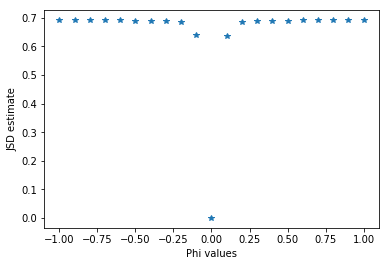
\includegraphics[scale=0.8]{jsd.png}
		\caption{JSD estimation}
		\label{fig:jsd}
	\end{figure}
	%
	\begin{figure}[H]
		\centering
		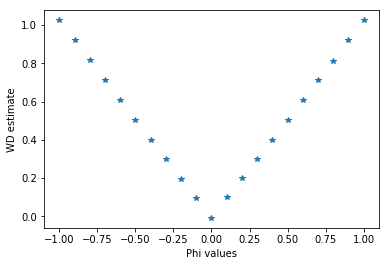
\includegraphics[scale=0.8]{wd.png}
		\caption{WD estimation}
		\label{fig:wd}
	\end{figure}
	%
	In this experiment the distributions $p$ and $q_\phi$ have disjoint supports for all values of $\phi$ but $\phi=0$. 
	As expected, the JSD when the distributions are disjoint is the same (around $\log(2)$) no matter how close the distributions may be i.e. for a small value of $\phi$. This results in a difficulty to learn the distribution $p$ using JSD. In contrast, WD is continuous over the values of $\phi$ giving a better information about the \emph{closeness} of the distributions.
	
	The full code is given in the file \textbf{density\_estimation.py} in our github repository~\cite{github}.

\item In this section we estimate the unknown density $f_1$ using the approximation ${f_0(x){D(x)}/(1-D(x))}$ (proven in Question 5 from the theoretical part), where $f_0$ is a known distribution (assumed 1-dimensional standard Gaussian in this question). The full code is provided in the file \textbf{density\_estimation.py} under our github repository~\cite{github}.

Using the above neural network (discriminator), we minimize the following function:
$$loss = -(torch.mean(torch.log(Dx)) + torch.mean(torch.log(1-Dy))),$$
where Dx is the feedforward of $f_1$ and Dy is the feedforward of $f_0$. 

The following figures show the discriminator's output and the estimated density:

\begin{figure}[H]
	\centering
	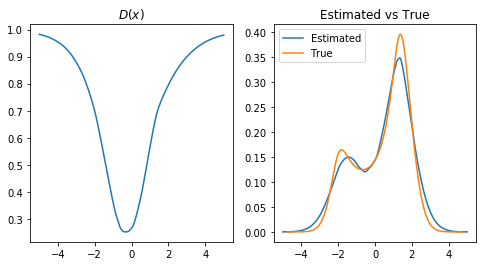
\includegraphics[scale=0.8]{disc.png}
	\caption{(left) Discriminator output (Right)Estimated $f_1$}
	\label{fig:disc}
\end{figure}



\end{enumerate}

